\documentclass[12pt]{article}
\usepackage{fullpage,enumitem,amsmath,amssymb,graphicx,amsthm,geometry,graphicx}

\geometry{left=2cm, right=2cm}

\begin{document}

\begin{center}
{\Large CS221 Fall 2017 Homework [Foundations]}

\begin{tabular}{rl}
Name: & yf-yang
\end{tabular}
\end{center}

By turning in this assignment, I agree by the Stanford honor code and declare
that all of this is my own work.

\section*{Problem 1}

\begin{enumerate}[label=(\alph*)]
  \item
    \small
      \begin{tabular}{||c|c|c|c|c|c||}
        \hline
          Input Vector & Weight & Out & Label & Loss & Grad w.r.t. Input \\
        \hline
        \hline
          $\begin{bmatrix}
            1 & 0 & 1 & 0 & 0 & 0
          \end{bmatrix}$
          &
          $\begin{bmatrix}
            0 & 0 & 0 & 0 & 0 & 0
          \end{bmatrix}$
          & 0 & -1 & 1 &
          $\begin{bmatrix}
            1 & 0 & 1 & 0 & 0 & 0
          \end{bmatrix}$ \\
        \hline
          $\begin{bmatrix}
            0 & 1 & 0 & 1 & 0 & 0
          \end{bmatrix}$
          &
          $\begin{bmatrix}
            -1 & 0 & -1 & 0 & 0 & 0
          \end{bmatrix}$
          & 0 & 1 & 1 &
          $\begin{bmatrix}
            0 & -1 & 0 & -1 & 0 & 0
          \end{bmatrix}$ \\
        \hline
          $\begin{bmatrix}
            0 & 1 & 0 & 0 & 1 & 0
          \end{bmatrix}$
          &
          $\begin{bmatrix}
            -1 & 1 & -1 & 1 & 0 & 0
          \end{bmatrix}$
          & 1 & -1 & 2 &
          $\begin{bmatrix}
            0 & 1 & 0 & 0 & 1 & 0
          \end{bmatrix}$ \\
        \hline
          $\begin{bmatrix}
            1 & 0 & 0 & 0 & 0 & 1
          \end{bmatrix}$
          &
          $\begin{bmatrix}
            -1 & 0 & -1 & 1 & -1 & 0
          \end{bmatrix}$
          & -1 & 1 & 2 &
          $\begin{bmatrix}
            -1 & 0 & 0 & 0 & 0 & -1
          \end{bmatrix}$ \\
        \hline
      \end{tabular}\\
    After the 4th backward propagation, we get a weight vector
    $ \mathbf{w} = 
    \begin{bmatrix}
      0 & 0 & -1 & 1 & -1 & 1
    \end{bmatrix}$. \qed
  
  \item
    Here are the four mini-reviews:\\
    \begin{center}
    \begin{tabular}{||c|c|c||}
      \hline
        Review & Vector & Label \\
      \hline
      \hline
        good & 
        $\begin{bmatrix}
            1 & 0 & 0
        \end{bmatrix}$
        & 1 \\
      \hline
        bad & 
        $\begin{bmatrix}
            0 & 1 & 0
        \end{bmatrix}$
        & -1 \\
      \hline
        not good & 
        $\begin{bmatrix}
            1 & 0 & 1
        \end{bmatrix}$
        & -1 \\
      \hline
        not bad & 
        $\begin{bmatrix}
            0 & 1 & 1
        \end{bmatrix}$
        & 1 \\
      \hline
    \end{tabular}
    \end{center}
    Thus, we can generate a system of four inequalities:
    \begin{equation}
      \begin{cases}
        w_1 \ge 1 \\
        w_2 \le -1 \\
        w_1 + w_3 \le -1 \\
        w_2 + w_3 \ge 1
      \end{cases}
    \end{equation}
    From which we have\\
      \begin{equation}
        \begin{cases}
          1 \le w_1 \le -1 - w_3 \\
          1 - w_3 \le w_2 \le -1    
        \end{cases}
      \end{equation}
    As a result
      \begin{equation}
        2 \le w_3 \le -2
      \end{equation}
    Which is impossible. The problem arises from interaction between not and other features. In order to fix this, we can add a feature "not good", then a weight vector like $
      \begin{bmatrix}
            1 & -1 & 2 & -4
      \end{bmatrix}$
    can achieve 0 error on the tiny dataset. \qed
    
\end{enumerate}

\section*{Problem 2}    
\begin{enumerate}[label=(\alph*)]
  \item
    \begin{equation}
        L(x, y, \mathbf{w}) = (y - \frac{1}{1+\exp({-\mathbf{w}\cdot\phi(x)})})^2
    \end{equation} \qed
  
  \item
    \begin{align}
      \frac{\partial L}{\partial\mathbf{w}} &= \frac{\partial L}{\partial p}\frac{\partial p}{\partial \mathbf{w}} \\
      &= -2(y-p)\phi(x)p^2\exp({-\mathbf{w}\cdot\phi(x)}) \\
      &= -2p(1-p)(y-p)\phi(x)
    \end{align} \qed
    
  \item
    The gradient is nearly 0 when p approaches 0 or 1, which means
    \begin{equation}
      \exp{(-\mathbf{w}\cdot\phi(x))} = +\infty \: or \: 0
    \end{equation}
    i.e.
    \begin{equation}
      \mathbf{w}\cdot\phi(x) = -\infty \: or \: +\infty
    \end{equation}
    Intuitively, when weights of $+1$ in $x$ approach $+\infty/-\infty$ and weights of $-1$ in $x$ approach $-\infty/+\infty$, the gradient would be very small. \qed

  \item
    When $p=\frac{1}{3}$, the gradient has the largest magnitude of $\frac{8}{27}\phi(x)$ \qed
    
  \item
    If I understand the problem correctly, then we have some $\mathbf{w}$ which satisfies
    \begin{equation}
      y = \frac{1}{1+\exp{(-\mathbf{w}\cdot\phi(x))}}
    \end{equation}
    for each (x, y) pairs in D.\\
    Thus.
    \begin{equation}
      \exp{(-\mathbf{w}\cdot\phi(x))} = \frac{1-y}{y}
    \end{equation}
    \begin{equation}
      \mathbf{w}\cdot\phi(x) = -\log{\frac{1-y}{y}}=log{y}-\log{(1-y)}
    \end{equation}
    Then, we can let
    \begin{equation}
      y'=log{y}-\log{(1-y)}
    \end{equation}
    The new label could be easily fitted with least squares regression. \qed

\end{enumerate}

\section*{Problem 3}    
\begin{enumerate}[label=(\alph*)]
  \setcounter{enumi}{3}
  \item
    \begin{enumerate}[label=\arabic*.]
    \item
      \begin{quote}
      screenwriter dan schneider and director shawn levy substitute volume and primary colors for humor and bite . \\
Truth: -1, Prediction: 1 [WRONG] \\
and                         3 * 0.17 = 0.51 \\
substitute                    1 * 0.08 = 0.08 \\
.                             1 * 0.08 = 0.08 \\
screenwriter                  1 * 0.03 = 0.03 \\
volume                        1 * 0 = 0 \\
shawn                         1 * 0 = 0 \\
primary                       1 * 0 = 0 \\
dan                           1 * 0 = 0 \\
humor                         1 * -0.02 = -0.02 \\
director                      1 * -0.02 = -0.02 \\
for                           1 * -0.04 = -0.04 \\
levy                          1 * -0.09 = -0.09 \\
bite                          1 * -0.09 = -0.09 \\
colors                        1 * -0.1 = -0.1 \\
schneider                     1 * -0.26 = -0.26
      \end{quote}
    Analysis: Some neutral words, especially "and", has a positive weight as high as .17, that may stem from our biased data set with more positive examples than negative examples. Besides, the occurrence frequency of "and" shouldn't be linear with out final output. It's problematic to multiply the weight of and directly by 3.
    \item  
      \begin{quote}
        a heady , biting , be-bop ride through nighttime manhattan , a loquacious videologue of the modern male and the lengths to which he'll go to weave a protective cocoon around his own ego . \\
Truth: 1, Prediction: -1 [WRONG] \\
ride                          1 * 0.88 = 0.88 \\
modern                        1 * 0.23 = 0.23 \\
ego                           1 * 0.19 = 0.19 \\
and                           1 * 0.17 = 0.17 \\
.                             1 * 0.08 = 0.08 \\
he'll                         1 * 0.07 = 0.07 \\
,                             3 * 0.02 = 0.06 \\
of                            1 * 0.05 = 0.05 \\
a                             3 * 9.95731275211e-16 = 2.98719382563e-15 \\
cocoon                        1 * 0 = 0 \\
videologue                    1 * 0 = 0 \\
loquacious                    1 * 0 = 0 \\ 
lengths                       1 * 0 = 0 \\ 
protective                    1 * 0 = 0 \\
weave                         1 * 0 = 0 \\ 
nighttime                     1 * 0 = 0 \\ 
be-bop                        1 * 0 = 0 \\
heady                         1 * -0.01 = -0.01 \\
biting                        1 * -0.06 = -0.06 \\
own                           1 * -0.08 = -0.08 \\
manhattan                     1 * -0.08 = -0.08 \\
through                       1 * -0.1 = -0.1 \\
go                            1 * -0.15 = -0.15 \\
his                           1 * -0.17 = -0.17 \\
which                         1 * -0.21 = -0.21 \\
the                           2 * -0.11 = -0.22 \\
to                            2 * -0.11 = -0.22 \\
male                          1 * -0.31 = -0.31 \\
around                        1 * -0.38 = -0.38
      \end{quote}
    Analysis: Some bias in out data set makes the weight of ride exceptionally high.
    \item
      \begin{quote}
        'it's painful to watch witherspoon's talents wasting away inside unnecessary films like legally blonde and sweet home abomination , i mean , alabama . ' \\
Truth: -1, Prediction: 1 [WRONG] \\
sweet                         1 * 0.56 = 0.56 \\
painful                       1 * 0.3 = 0.3 \\
home                          1 * 0.22 = 0.22 \\
films                         1 * 0.21 = 0.21 \\
and                           1 * 0.17 = 0.17 \\
.                             1 * 0.08 = 0.08 \\ 
blonde                        1 * 0.07 = 0.07 \\
legally                       1 * 0.07 = 0.07 \\
inside                        1 * 0.05 = 0.05 \\ 
i                             1 * 0.05 = 0.05 \\
alabama                       1 * 0.04 = 0.04 \\ 
,                             2 * 0.02 = 0.04 \\
wasting                       1 * 0 = 0 \\
abomination                   1 * 0 = 0 \\
'it's                         1 * 0 = 0 \\
witherspoon's                 1 * 0 = 0 \\
away                          1 * -0.04 = -0.04 \\
mean                          1 * -0.06 = -0.06 \\
talents                       1 * -0.07 = -0.07 \\ 
to                            1 * -0.11 = -0.11 \\
like                          1 * -0.15 = -0.15 \\
unnecessary                   1 * -0.15 = -0.15 \\
watch                         1 * -0.15 = -0.15 \\
'                             1 * -0.17 = -0.17
      \end{quote}
    Analysis: The word "like" has interaction with examples behind, so words like "sweet" should not affect our result. Besides, I don't know why "painful" has a positive weight.
    \item
      \begin{quote}
        wickedly funny , visually engrossing , never boring , this movie challenges us to think about the ways we consume pop culture . \\
Truth: 1, Prediction: -1 [WRONG] \\
culture                       1 * 0.43 = 0.43 \\
funny                         1 * 0.42 = 0.42 \\
ways                          1 * 0.3 = 0.3 \\
us                            1 * 0.23 = 0.23 \\
wickedly                      1 * 0.22 = 0.22 \\
engrossing                    1 * 0.22 = 0.22 \\
visually                      1 * 0.1 = 0.1 \\
.                             1 * 0.08 = 0.08 \\
think                         1 * 0.07 = 0.07 \\
,                             3 * 0.02 = 0.06 \\ 
challenges                    1 * 0.05 = 0.05 \\
we                            1 * 0.05 = 0.05 \\
consume                       1 * 0 = 0 \\
this                          1 * -5.89805981832e-17 = -5.89805981832e-17 \\
movie                         1 * -0.09 = -0.09 \\
the                           1 * -0.11 = -0.11 \\
about                         1 * -0.11 = -0.11 \\
to                            1 * -0.11 = -0.11 \\
pop                           1 * -0.24 = -0.24 \\
never                         1 * -0.37 = -0.37 \\
boring                        1 * -1.26 = -1.26
      \end{quote}
    Analysis: The stupid linear predictor can't understand interaction between "never" and "boring".
    \item
      \begin{quote}
        atchy combination of soap opera , low-tech magic realism and , at times , ploddingly sociological commentary . \\
Truth: -1, Prediction: 1 [WRONG] \\
magic                         1 * 0.54 = 0.54 \\
realism                       1 * 0.42 = 0.42 \\
times                         1 * 0.24 = 0.24 \\
and                           1 * 0.17 = 0.17 \\
at                            1 * 0.08 = 0.08 \\ 
.                             1 * 0.08 = 0.08 \\
,                             3 * 0.02 = 0.06 \\
of                            1 * 0.05 = 0.05 \\ 
sociological                  1 * 0.02 = 0.02 \\
patchy                        1 * 0 = 0 \\
ploddingly                    1 * 0 = 0 \\
low-tech                      1 * 0 = 0 \\
combination                   1 * -0.11 = -0.11 \\
commentary                    1 * -0.2 = -0.2 \\
opera                         1 * -0.3 = -0.3 \\
      \end{quote}
    Analysis: Our predictor haven't encountered "low-tech" before and can't understand relations between "low-tech" and "magic realism".
    \end{enumerate} \qed
    \setcounter{enumi}{5}
    \item 
      See prob3-6.py for the code, the result is demonstrated in Fig 1. \\
      \begin{figure}
          \centering
          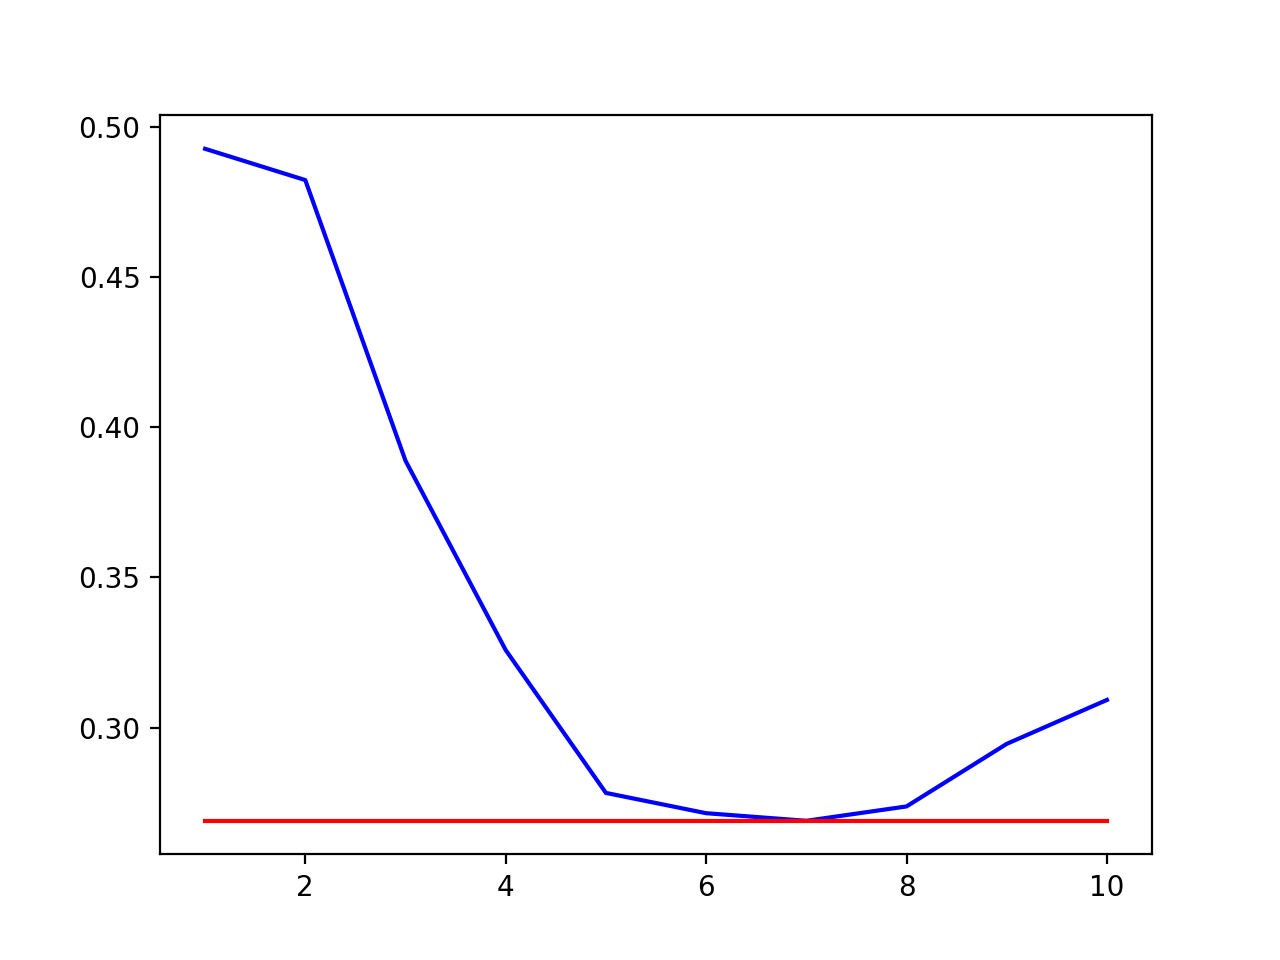
\includegraphics{fig3_6.png}
          \caption{Character Features(blue) vs Word Features(red)}
      \end{figure}
      Analysis: When $n \approx 7$, our predictor achieves the best result. That's because ~7 characters could contain a word and some interaction between the word and previous/next one, while the noise introduced by bilateral words are not so high. \qed
      
\end{enumerate}

\section*{Problem 4}    
\begin{enumerate}[label=(\alph*)]
  \item 
    \begin{enumerate}[label=\arabic*.]
        \item
        \# assign point 2, 4 to center 1, assign point 1, 3 to center 2 \\
        \# get new centers $ \mu_1 = [.5, 2], \mu_2=[1, 0]$ \\
        \# assign point 2, 4 to center 1, assign point 1, 3 to center 2 \\
        \# convergence
        \item
        \# assign point 1, 2 to center 1, assign point 3, 4 to center 2 \\
        \# get new centers $ \mu_1 = [0, 1], \mu_2=[1.5, 1]$ \\
        \# assign point 1, 2 to center 1, assign point 3, 4 to center 2 \\
        \# convergence
    \end{enumerate}\qed
  \setcounter{enumi}{2}
  \item
    \begin{enumerate}[label=\arabic*.]
      \item Get M connected components based on S (note that a single vertex is also an connected component), assure $M \ge K$.
      \item If a connected component has more than 1 vertices, we use it's center of mass as it's coordinate. Then, randomly sample K connected components and use it's coordinate as initial centers.
      \item If a connected component has more than 1 vertices, we use the vertices' average distance from a point as the distance between the connected component and that point. Then, assign each connected components to it's nearest center.
      \item stop if the process converges, otherwise go back to step 2. \qed
    \end{enumerate}
\end{enumerate}

\end{document}
